\section{Pictogram Endpoint}\label{pictogramendpoint}
This section will solve the \userstory{As a developer I would like an endpoint for Pictograms, such that I can retrieve them from GIRAF.}

The Pictogram endpoint is used for the PictoSearch library to find different pictograms, as well as to acquire specific pictograms which have not been downloaded yet.
Currently in the PictoSearch library a user searches for some string, and the local database is queried using \texttt{... LIKE \%searchstring\%} and as such this will also be used for the REST API.
Therefore a goal of the REST API for pictograms is to provide a search method, such that PictoSearch will return the same results.
The endpoint will also be used in the case that a user opens e.g. a week schedule which contains a pictogram that the device have not stored locally, the endpoint will then retrieve this single pictogram rather than returning a list of pictograms.

\subsection{Description of the Model of Pictograms}\label{subsec:pictomodel}
The model that was described in \myref{subsec:model} was the complete model of the REST API, \myref{fig:pictogramModel} shows the model regarding pictograms along with the fields of these classes.

\begin{figure}[h]
    \centering
    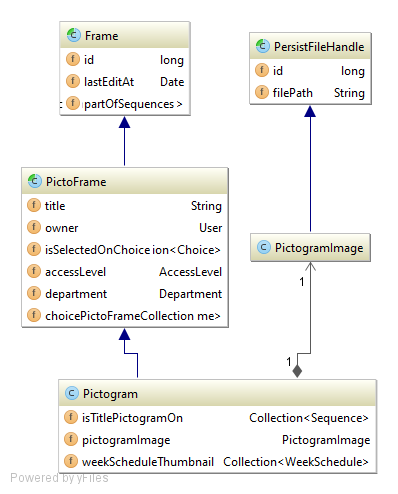
\includegraphics[width=0.5\textwidth]{figures/diagram-pictogram.png}
    \caption{Class--diagram including fields of the classes involved in Pictograms}\label{fig:pictogramModel}
\end{figure}\todo{Update accordingly in the end}

\todo{Table or description? --- I will make consistent when we decide}
Here a brief description of the purpose for each field of the classes on the figure will be given.
\subsubsection*{Frame}
	\begin{description}
		\item[id] This is the id of the Frame which is saved in the database.
		\item[lastEditAt] This is a time stamp of when the Frame was last edited --- auto updated by Hibernate when changes on the object is persisted in the database.
		It is to be used for conflict handling as e.g. pictograms can be altered in the PictoCreator tool, and a need for conflict handling is therefore needed.
		\item[partofSequences] This is a collection of sequences this frame is used in; why this collection is needed will be further explained in \todo[inline]{sequenceendpointref}
	\end{description}

\subsubsection*{PictoFrame}
	\begin{description}
		\item[title] Title of the \texttt{PictoFrame}. Is used to search for and also to show what the \texttt{PictoFrame} is called when shown with its title in different parts of GIRAF.
		\item[owner] The user which owns the \texttt{PictoFrame}, but not necessarily the user whom created it.
		This is used to accommodate the need for creating private \texttt{Pictograms} and \texttt{Sequences}.
		Private means that only the user who is owner can access them.
		\item[accessLevel] This is an Enumeration which specifies whether the \texttt{PictoFrame} is Public, shared on department or private.
		\item[department] Specifies which department the \texttt{PictoFrame} belongs to, and is used when the accessLevel is specified as shared on department.
		\item[optionOn] A collection of all \texttt{Choice}s which contain the \texttt{PictoFrame}.
		This is needed for Hibernate to create the many-to-many relationship between \texttt{PictoFrame} and \texttt{Choice}, and will probably not be used for anything else.
	\end{description}

\subsubsection*{Pictogram}
	\begin{description}
		\item[isTitlePictogramOn] A collection of the \texttt{Sequence}s which this \texttt{Pictogram} is the titlePictogram of.
		\item[pictogramImage] A reference to the \texttt{PictogramImage} of the \texttt{Pictogram}.
		\item[weekScheduleThumbnail] Similar to the \texttt{isTitlePictogramOn} but this is for a collection of \texttt{WeekSchedule}s instead.
	\end{description}

\subsubsection*{PictogramImage}
The \texttt{PictogramImage} has no fields of its own, but is used to indicate that the image is used for a \texttt{Pictogram} instead of e.g. a UserIcon.
However it inherits fields for PersistFileHandle.

\subsubsection*{PersistFileHandle}
This class is what all objects that encapsulates image files will inherit from, this means \texttt{PictogramImage}s and also \texttt{UserIcon}s.
Originally when we started working on the REST API for Pictogram the \texttt{PersistFileHandle} did not exist and all information on this class was saved directly on the \texttt{UserIcon} class.
Why and how this new generality is created will be explained in \myref{subsec:persistfilehandle}.
It contains the following fields:
\begin{description}
	\item[id] This field is self explanatory.
	\item[filePath] A string of the path to the file which the class points to, for the Pictogram endpoint it will be a Pictogram.
\end{description}

The section above explains what is modelled with the Java classes; the following section will present how this information is stored in the database using the tools mentioned in \myref{sec:techstack}.

\subsection{Storing the Model in the Database}

As mentioned previously we use an \textbf{ORM} (object--relational mapping) tool to map the models to the database, this section describes how this specifically is done.

\begin{lstlisting}[float, floatplacement=h, caption={Fields with annotations which causes Hibernate to perform the ORM for a \texttt{PictogramImage}.},label={lst:PictoImage}]
@OneToOne(fetch = FetchType.LAZY, cascade = CascadeType.ALL, optional = true)
private PictogramImage pictogramImage;
\end{lstlisting}

The short snippet in \myref{lst:PictoImage} shows how the relation to the \texttt{PictogramImage} is created in the \texttt{Pictogram} class.
It simply uses the \texttt{@OneToOne} annotation to create the One-to-One relation between these two objects.
This is only done on the \texttt{Pictogram} and not on the side of the \texttt{PictogramImage}.
The property \texttt{fetch} is sat to \texttt{LAZY} which means that the \texttt{PictogramImage} is not retrieved in the same transaction as when the \texttt{Pictogram} is retrieved, but is instead retrieved when the \texttt{PictogramImage} is accessed through the \texttt{Pictogram} object.
The other fetch type \texttt{EAGER} would instead retrieve the entity in the same transaction as the \texttt{Pictogram}.
The \texttt{CascadeType.All} means that any change which happens to the \texttt{Pictogram} must cascade to \texttt{PictogramImage} as well.
The field is set to being optional because when creating the \texttt{Pictogram} using a HTTP POST request, you cannot send the JSON data along with the image file, and as such the requests have to be separated into two.
The field is therefore optional to allow for the \texttt{Pictogram} to exist without the \texttt{PictogramImage} for a while, as we deemed it better that a \texttt{Pictogram} exists without a \texttt{PictogramImage} than vice versa.

When creating a One-to-Many a opposite Many-to-One needs to be created on the class the relation is created to.

This needs to be done for the field \texttt{isTitlePictogramOn} as can be seen on \myref{lst:titlePictogram}.

\begin{lstlisting}[float, floatplacement=h, caption={Fields with annotations which causes Hibernate to perform the ORM for \texttt{titlePictogram}. \texttt{[...]} denotes omitted code.},label={lst:titlePictogram}]
//The relation on the side of Sequence
public class Sequence extends PictoFrame implements Iterable<Frame> {
	[...]
	@ManyToOne(fetch = FetchType.EAGER)
	@JoinColumn(name = "titlePictogram_id")
	private Pictogram titlePictogram;
	[...]
}
// The relation on the side of Pictogram
public class Pictogram extends PictoFrame {
	[...]
    @OneToMany(fetch = FetchType.LAZY)(*@\label{lst:tp_rel_on_pictog1}@*)
	private Collection<Sequence> titlePictogramOn;(*@\label{lst:tp_rel_on_pictog2}@*)
	[...]
}
// SQL for the Sequence Schema
CREATE TABLE Sequence
(
    frame_id BIGINT NOT NULL PRIMARY KEY,
    titlePictogram_id BIGINT NOT NULL(*@\label{lst:tp_sql_meme}@*)
);
\end{lstlisting}

On line 5 the \texttt{@JoinColumn} Hibernate annotation is used to specify which column the two tables \texttt{Pictogram} and \texttt{Sequence} will join on.
Lines~\ref{lst:tp_rel_on_pictog1}--\ref{lst:tp_rel_on_pictog2} shows the relation needed on the side of \texttt{Pictogram} to create the opposite One-to-Many side to the Many-to-One relationship on \texttt{Sequence}.
Line~\ref{lst:tp_sql_meme} shows the SQL where the column to be joined on is created in the SQL.

\subsection{Querying the Database}
As explained in \myref{subsec:general} the database is queried using a DAO, this section will present the \texttt{PictogramDaoImpl} class.

\begin{lstlisting}[float, floatplacement=h, caption={The class header of the \texttt{PictogramDao}, along with its annotations. \texttt{[...]} denotes omitted code.},label={lst:pictogramDaoImpl}]
@Transactional
@Repository
@Primary
public class PictogramDaoImpl extends BaseDaoImpl<Pictogram> implements PictogramDao {
	[...]
}
\end{lstlisting}

\myref{lst:pictogramDaoImpl} shows the class header of the \texttt{PictogramDaoImpl}, it extends \texttt{BaseDaoImpl<Pictogram} and implements its relating interface \texttt{PictogramDao} as described in \myref{subsec:general}.
It has the annotation \texttt{@Transactional} which is a Spring annotation all DAOs in the REST API use.
It allows Spring to inject behaviours around method calls like transaction management.
The \texttt{@Reposity} annotation is also a Spring annotation used for all DAOs in the REST API, which tells spring that the class is used for encapsulating storage, retrieval and search behaviour for a collection of objects.
The last annotation \texttt{@Primary} is also a Spring annotation used by all DAOs in the REST API, and is used to tell Spring that the Java Bean \todo{Det har vi vel ikke nævnt?} containing this class should be given preference when multiple beans are candidates to be autowired.
Autowire means that you do not have to specify the bean's properties or constructor arguments explicitly.
This is used in the Service layer where the proper DAOs are retrieved as Beans and the auto wiring makes this easier.

\bigskip
\myref{lst:pictogramByTitle} shows the method for querying the database for \texttt{Pictogram}s which title contains the string being searched for.
Lines~\ref{lst:pictogrambt_tq1}--\ref{lst:pictogrambt_tq2} creates a \texttt{TypedQuery} which uses the \texttt{LIKE} operator to find any \texttt{Pictogram} which title adheres to the pattern \texttt{:title}.
Line~\ref{lst:pictogrambt_tq3} then sets \texttt{:title} to be any string concatenated with the search string, which is then concatenated by any string as well.
\begin{lstlisting}[float, floatplacement=h, caption={The method which searches through all \texttt{Pictogram}s by their titles.},label={lst:pictogramByTitle}]
    /**
     * Search for public pictograms by title.
     *
     * @param title to search for (substring of real title)
     * @return pictograms whose title include the query
     */
    @Override
    public Collection<Pictogram> searchByTitle(String title) {
        TypedQuery<Pictogram> query = em.createQuery("SELECT p FROM Pictogram p " +(*@\label{lst:pictogrambt_tq1}@*)
            "WHERE (p.title LIKE :title) " +
            "AND p.accessLevel = :public", Pictogram.class);(*@\label{lst:pictogrambt_tq2}@*)
        query.setParameter("title", "%" + title + "%");(*@\label{lst:pictogrambt_tq3}@*)
        query.setParameter("public", AccessLevel.PUBLIC);
        return query.getResultList();
    }
\end{lstlisting}

As mentioned in \myref{subsec:general}, the persistence layer is tested, which means that the method \texttt{SearchByTitle} is also tested --- the test for this method can be seen on \myref{lst:pictogramByTitleTest}.
It starts by assigning what is returned by the \texttt{searchByTitle} method to an \texttt{ArrayList} on line~\ref{lst:tpbt_1love}.
lines~\ref{lst:tpbt_2loves}--\ref{lst:tpbt_3loves} asserts first if the results is empty, followed by asserting whether the \texttt{ArrayList} contains a specific \texttt{Pictogram}.
The rest of the asserts check whether the \texttt{PictogramImage} is also as expected, which essentially tests whether Hibernate retrieves the \texttt{Pictogram}'s one-to-one relation correctly.

\begin{lstlisting}[float, floatplacement=h, caption={The test method which tests the method \texttt{SearchByTitle}.},label={lst:pictogramByTitleTest}]
@Test
public void testPictogramByTitle() throws Exception {
    ArrayList<Pictogram> pictogramlist = new ArrayList<Pictogram>(pictogramDao.searchByTitle("test1"));(*@\label{lst:tpbt_1love}@*)

    Assert.assertFalse(pictogramlist.isEmpty());(*@\label{lst:tpbt_2love}@*)
    Assert.assertTrue(pictogramlist.stream()
    	.anyMatch(p -> p.getId() == 1L));

    Assert.assertTrue(pictogramlist.stream()
    	.anyMatch(p -> p.getPictogramImage().getFilePath().equals("jeff")));
    Assert.assertTrue(pictogramlist.stream()
    	.anyMatch(p -> p.getPictogramImage().getId() == 1L));(*@\label{lst:tpbt_3love}@*)
}
\end{lstlisting}

\subsection{Generalising the FileDAO}\label{subsec:persistfilehandle}
When we started working on the REST API \texttt{Pictogram}, there was already created a way to get an image in another class, namely the \texttt{UserIcon}.
A DAO was also created for \texttt{UserIcon}, which contained methods which were the exact same methods we needed to implement for the \texttt{PictogramImage}, so to avoid \enquote{copy--paste} code we decided to generalise the concept.
This is when the class \texttt{PersistFileHandle} was created as mentioned in \myref{subsec:pictomodel}.
It meant that the data was now inherited from a single class.
When creating a DAO for retrieving the information we did not want to copy--paste as well, as the queries would retrieve the same data just for different kind of objects, therefore the DAO was generalised using Type parameters as shown on \myref{lst:typeparameter}.
This means that any Type that extends from the class \texttt{PersistFileHandle} is able to be used with this Class, which means that both \texttt{PictogramImage} and \texttt{UserIcon} can now be used.

\begin{lstlisting}[float, floatplacement=h, caption={The \texttt{FileDaoImpl} class header which uses Type Parameters to generalise which types it can be used with. \texttt{[...]} denotes omitted code.},label={lst:typeparameter}]
public abstract class FileDaoImpl<T extends PersistFileHandle> implements FileDao<T> {
	[...]
}
\end{lstlisting}

As we started to generalise the methods in \texttt{FileDaoImpl} we faced a problem in the \texttt{add} method as we created a new object using a constructor, which would now be the type parameter \texttt{T} as seen on \myref{lst:TypeParameterConstructor}.
Therefore we decided to use the abstract factory pattern, such that the method knows exactly what object it needs to use.
For further reading on the factory pattern see The Gang of Four's description in their book \textit{Design Patterns: Elements of Reusable Object-oriented Software} \cite{abstractfactorypattern}.
The \textit{Abstract Factory Pattern} can be shown using our own classes on \myref{fig:asbtractFactory}.

\begin{lstlisting}[float, floatplacement=h, caption={Trying to use a Type Parameter constructor, which Java cannot do. \texttt{[...]} denotes omitted code.},label={lst:TypeParameterConstructor}]
public T add(Readable file) throws IOException {
    [...]
    T fh = new T(uuid.toString());
    [...]
}
\end{lstlisting}

\begin{figure}[h]
    \centering
    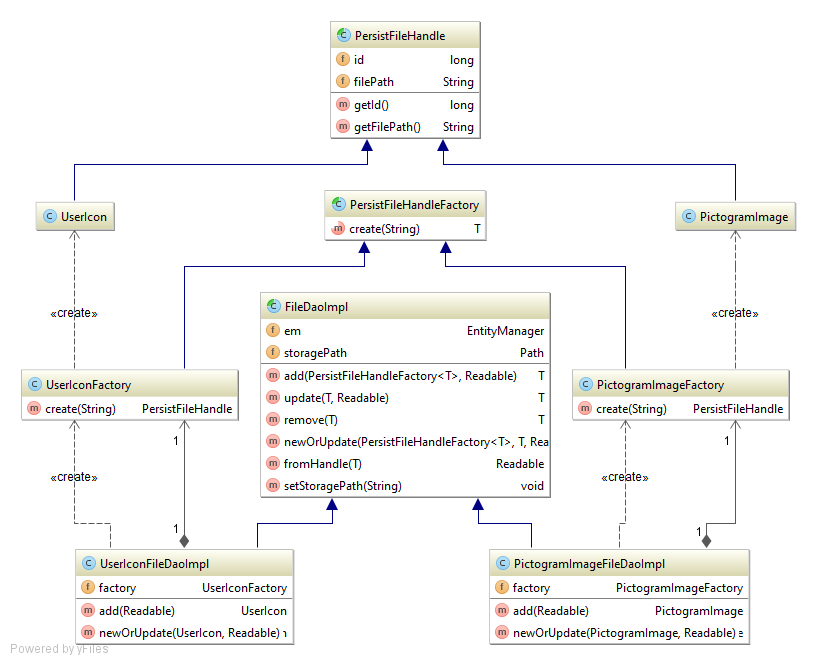
\includegraphics[width=0.5\textwidth]{figures/diagram-factory.png}
    \caption{The abstract factory pattern in the REST API for \texttt{PersistentFileHandle}.}\label{fig:asbtractFactory}
\end{figure}

The abstract factory or factory of factories is the \texttt{PersistFileHandleFactory}.
When e.g. a \texttt{FileDao<PictogramImage>} is created, an instance of \texttt{pictogramImageFileDaoImpl} is what is actually created.
This instance has a factory field, which will then be one of the non abstract subclasses or subfactories of \texttt{PersistFileHandleFactory} which in this case is the \texttt{PictogramImageFactory}.
This means that the \texttt{add} function mentioned earlier now knows what object it is working on and thus the line shown in \myref{lst:TypeParameterConstructor} can be changed to the line shown in \myref{lst:TypeParameterConstructorActual}.

\begin{lstlisting}[float, floatplacement=h, caption={Trying to use a Type Parameter constructor, which Java cannot do. \texttt{[...]} denotes omitted code.},label={lst:TypeParameterConstructorActual}]
public T add(PersistFileHandleFactory<T> factory, Readable file) throws IOException {
    [...]
      fh = factory.create(uuid.toString());
    [...]
}
\end{lstlisting}

Using this pattern the factory, whatever type it may be, has a create method which takes a string as input.
The factory variable will either be a \texttt{UserIconFactory} or a \texttt{PictogramImageFactory}, where the create methods both create their corresponding class with the path set to the string that is sent as input.
In this way the pattern of storing files and the paths to the files is generalised, and can work for virtually any other type of file, as long as they implement a factory which inherit from the abstract factory, and a class which inherits from the abstract class \texttt{PersistFileHandle}.

\subsection{The Service Layer for the Pictogram}
This section describes the service layer of the Pictogram endpoint.
The tool RESTEasy makes it simple to create HTTP Request methods using its annotations such as \texttt{@GET} or \texttt{@PUT}.
\myref{tbl:pictogramservice} shows a list of all the services provided by the pictogram REST API.
All the services are located in the path \texttt{/publicpictogram} and \texttt{/department/\{id\}/pictogram}.
This separation has been made because the public pictograms are all given by the GIRAF application, while the other pictograms are pictograms that will be created by a department.

\begin{table}[]
\footnotesize
\centering
\begin{tabular}{rll}
HTTP Request    & Path          & Method Name                   \\
\midrule
GET             &/              & \texttt{getAllPictograms}     \\
GET             &/\{pid\}       & \texttt{getPictogram}         \\
GET             &/\{pid\}/image & \texttt{getPictogramImage}    \\
\tblgrpsep
POST            &/              & \texttt{CreatePictogram}      \\
\tblgrpsep
PUT             &/\{pid\}/image & \texttt{uploadPictogramImage} \\
PUT             &/\{pid\}       & \texttt{updatePictogram}      \\
\tblgrpsep
DELETE          &/\{pid\}	    & \texttt{deletePictogram}	    \\
\end{tabular}
\caption{List of Pictogram endpoints, they all exist at \texttt{/department/\{id\}/pictogram} or at \texttt{/publicpictogram}.}\label{tbl:pictogramservice}
\end{table}

The services use the DAOs created in the persistence layer of the REST API.
The queries created in the DAO retrieve the objects that the request wants to either GET, PUT, or DELETE, otherwise for a POST request a builder for \texttt{Pictogram} will build the \texttt{Pictogram} from the JSON data, and the method that handles the request will then save this in the database.

\myref{lst:getallPictograms} shows the method which handles a GET request on the root path which is seen from the annotations \texttt{@GET} and \texttt{@Path("/")}.
Since a \texttt{PictogramService} is only created through the \texttt{DepartmentService} on the path \texttt{"/pictogram"} the full path to activate this method is \texttt{"department/\{id\}/pictogram/"}.
The annotation on line 8 simply states which representation a resource can produce in this case it means that this method can produce JSON as output.
The last annotation on line 9 \texttt{RolesAllowed({PermissionType.Constants.USER})}, specifies which roles may access this method, and \texttt{USER} is the most general one, which means every type of user in the model may access this method.

\begin{lstlisting}[float, floatplacement=h, caption={A GET request to get all pictograms for a department.},label={lst:getallPictograms}]
/**
 * Get a list of all the private/protected {@link Pictogram pictograms}. Any user of a department can do this.
 * @param user The currently authenticated user
 * @return A collection of {@link Pictogram pictograms}.
 */
@GET
@Path("/")
@Produces("application/json")
@RolesAllowed({ PermissionType.Constants.USER })
public Collection<Pictogram> getAllPictograms(@Context User user) {
    if(user == null)
        throw new NotAuthorizedException("You need to be logged in to add department pictograms");
    if(!user.getDepartment().equals(department) && !user.hasPermission(PermissionType.SuperUser))
        throw new NotAuthorizedException("You are logged in to the wrong department");

    return pictogramDao.getAll(user);
}
\end{lstlisting}

First, the method simply checks if a user is actually received, i.e. is a user logged in or not.
If this check passes the next if--check on line 13 checks whether the user is in the same department as the department the method will try to get \texttt{Pictogram}s from, if this check fails it also checks whether the user might be a \texttt{SuperUser}, in which case it is also allowed and the if--check will fail.
A \texttt{SuperUser} is a user with permissions to do administrative tasks such as create public pictograms.

If both if--checks fail, the method returns what the \texttt{PictogramDao.getAll(user)} method retrieves, which will be all pictograms the user is allowed to see.

This concludes the \texttt{Pictogram} endpoint showcase; the next section will cover how the REST API for \texttt{Sequence} was progressed for this sprint, it will skip details already covered in this section about the \texttt{Pictogram} endpoint.
